%%%%%%%%%%%%%%%%%%%%%%%%%%%%%%%%%%%%%%%%%
% Structured General Purpose Assignment
% LaTeX Template
%
% This template has been downloaded from:
% http://www.latextemplates.com
%
% Original author:
% Ted Pavlic (http://www.tedpavlic.com)
%
% Note:
% The \lipsum[#] commands throughout this template generate dummy text
% to fill the template out. These commands should all be removed when 
% writing assignment content.
%
%%%%%%%%%%%%%%%%%%%%%%%%%%%%%%%%%%%%%%%%%

\documentclass{article}

\usepackage{fancyhdr} % Required for custom headers
\usepackage{lastpage} % Required to determine the last page for the footer
\usepackage{extramarks} % Required for headers and footers
\usepackage{graphicx} % Required to insert images
\usepackage[utf8]{inputenc}

% Margins
\topmargin=-0.45in
\evensidemargin=0in
\oddsidemargin=0in
\textwidth=6.5in
\textheight=9.0in
\headsep=0.25in 

\linespread{1.1} % Line spacing



\setlength\parindent{0pt} % Removes all indentation from paragraphs

%----------------------------------------------------------------------------------------
%	DOCUMENT STRUCTURE COMMANDS
%	Skip this unless you know what you're doing
%----------------------------------------------------------------------------------------

% Header and footer for when a page split occurs within a problem environment
\newcommand{\enterProblemHeader}[1]{
\nobreak\extramarks{#1}{#1 continued on next page\ldots}\nobreak
\nobreak\extramarks{#1 (continued)}{#1 continued on next page\ldots}\nobreak
}

% Header and footer for when a page split occurs between problem environments
\newcommand{\exitProblemHeader}[1]{
\nobreak\extramarks{#1 (continued)}{#1 continued on next page\ldots}\nobreak
\nobreak\extramarks{#1}{}\nobreak
}

\setcounter{secnumdepth}{0} % Removes default section numbers
\newcounter{homeworkProblemCounter} % Creates a counter to keep track of the number of problems

%----------------------------------------------------------------------------------------
%	NAME AND CLASS SECTION
%----------------------------------------------------------------------------------------

\newcommand{\lessonNumber}[1]{Lezione\ \##1} % Assignment title
\newcommand{\lessonDate}[4]{#1,\ #2\ #3\ #4} % Due date
\newcommand{\lessonCourse}[1]{#1} % Course/class
\newcommand{\lessonTime}[1]{#1} % Class/lecture time
\newcommand{\lessonTeacher}[1]{#1} % Teacher/lecturer
\newcommand{\lessonAuthor}[1]{#1} % Your name

\begin{document}

\section{Il ciclo di vita del software(3)}
% Lunedì 14 Ottobre 2013

\textbf{Ciclo di vita di un software:} Evolve nel tempo e raggiunge \textbf{stati} tramite \textbf{transizioni} scatenate da attività che hanno il fine di far avanzare il sw. Si divide in 4 fasi:

\begin{itemize}

	\item \textbf{Concezione}, quando qualcuno pensa che ci sia (o abbia) bisogno di qualcosa;
	\item \textbf{Sviluppo};
	\item \textbf{Utilizzo};
	\item \textbf{Ritiro}.

\end{itemize}

\textbf{Fase}:\fbox{\textbf{Def} Periodo di tempo contiguo che cattura transizioni o segmenti di ciclo di vita}

La scelta del ciclo di vita pone vincoli sulla pianificazione del progetto, è indipendente da metodi e strumenti di sviluppo.\\

Tipi di ciclo di vita:
\begin{itemize}
	\item \textbf{Cascata:} successione di fasi rigidamente sequenziali con dipendenze causali tra di loro, non ammette ritorno a fasi precedenti.(Pre e Post solide e definite all'origine, modello che non spreca, al tempo t so dove sono). Modello \textbf{Document driven} (documenti che spiegano la fiducia nelle scelte fatte), non sono previsti prototipi.\\
	Difetti: eccessivamente rigido, non ammette cambiamenti ai requisiti in corso d'opera, il committente vede solo l'opera finita.
	\item \textbf{Incrementale:} modello iterativo, potenzialmente distruttivo(avanzo nel tempo ma non nei risultati). In questo modello procedo per fasi che possono anche essere completamente separate le une dalle altre, ma a differenza del waterfall posso integrare anche le piccole parti. Produco valore ad ogni incremento, ed ogni incremento riduce il rischio di fallimento; le funzionalità essenziali inoltre sono sviluppate nei primi incrementi.
	Qui si prevedono rilasci multipli e successivi(base stabile ed aggiungo successivamente). Non si ripetono mai l'analisi e la progettazione architetturale.
	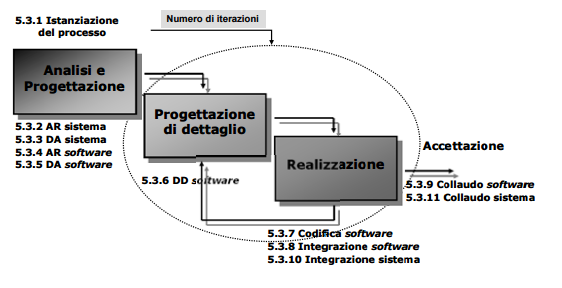
\includegraphics[width=0.75\columnwidth]{img4} % Example image
	\\Non ritorno mai sul progetto generale.\\
	
	\item \textbf{Iterativo:} comporta il rischio di non convergenza all'obbiettivo, tuttavia consentono maggior capacità di adattamento. Ogni iterazione comporta un ritorno all'indietro, nella direzione opposta rispetto al tempo.
	\item \textbf{Evolutivo:} insegue il futuro non ritirando il passato, ho tante attività concorrenti.Questo modello lo attua chi può sostenere molte versioni in parallelo (e quindi ha buone capacità finanziarie), infatti ogni fase ammette iterazioni multiple e parallele. Si può anche modificare la base ATT.
	\item\textbf{Spirale:} è composto da cicli interni rapidi e ripetuti, mentre quelli esterni aderiscono a qualsiasi altro modello std. Comporta un miglior controllo dei rischi di progetto, infatti pone molta attenzione sugli aspetti gestionali (pianificazione delle fasi, analisi dei rischi), è un modello \textbf{risk driven}. Prevede 4 attività principali 				 		\begin{itemize}
			\item Definizione degli obbiettivi
			\item Analisi dei rischi
			\item Sviluppo e validazione
			\item Pianificazione
		\end{itemize}
	Utilizzato solo per progetti innovativi
		
		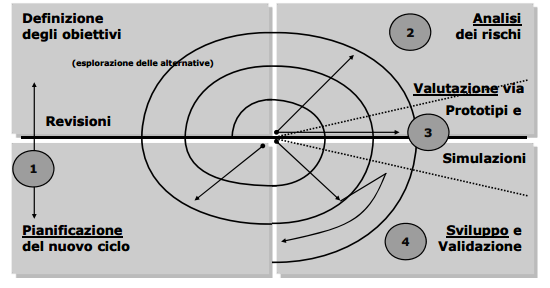
\includegraphics[width=0.75\columnwidth]{img5} % Example image
		\\
		I quadrati rappresentano dei macrostati.
		\item \textbf{Componenti:} si basa sul riuso dei componenti già fatti, utilizzo meno risorse ed ho un ecosistema(librerie e strumenti) già pronti.
	\item \textbf{Metodi Agili:} basati su 4 principi fondamentali:
	\begin{enumerate}

		\item Mettere in primo piano persone e iterazioni piuttosto che processi e strumenti. Gli individui sono importanti ed è importante il modo in cui interagiscono tra loro;
	
		\item ciò  che importa e che il sw funzioni non la documentazione;
	
		\item Avere un buon rapporto con il customer, coinvolgerlo;
	
		\item Reattività piuttosto che pianificazione. Capacità di adattamento a cambiamenti delle situazioni.

	\end{enumerate}
	L'idea base e di costruire degli user story che sono definiti da
		\begin{itemize}
			\item Un documento di descrizione;
			\item La minuta della conversazione con il cliente;
			\item Piano dei test per confermare che la strategia funziona.
		\end{itemize}
	Questi tipi di metodi permettono dunque di dimostrare costantemente ciò che e stato fatto, verificare l'avanzamento tramite progresso reale, assicurare che l'intero prodotto sw è ben verificato e integrato.
	\textbf{Scrum}, \textbf{Kanban} e \textbf{Scrumban} sono degli esempi.
\end{itemize}
\textbf{Scrum:} regole interne molte collaborative. Ci sono 3 tipi di fase:
	 \begin{itemize}
	 		\item Backlog: "le cose da fare", requisiti e funzionalità del prodotto;
	 		\item Spirit Backlog: insieme di storie del prossimo spirit
	 		\item Spirit: fase operativa di sviluppo, durata 2-4 settimane, alla fine abbiamo un prodotto potenzialmente vendibile.
	 \end{itemize}
Ad ogni periodo di tempo si prendono le cose più necessarie e si esegue uno spirit, non appena è terminatose manca qualcosa si ritorna al backlog aggiungendo \textit{to do}. Questo ciclo di vita e iterativo in quanto non ho un numero casuale di spirit e questi producono quasi sempre un avanzamento.

\textbf{SEMAT:} \\
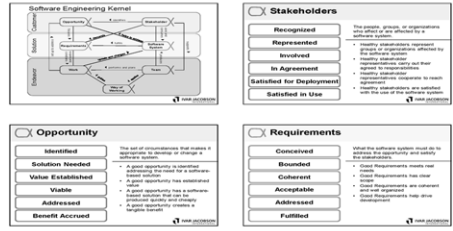
\includegraphics[width=0.5\columnwidth]{img6}\\
I \textit{Requirements} hanno 6 aggettivi:
\begin{itemize}
	\item \textbf{Conceived:} i requisiti vanno concepiti, nascono nel luogo dove stanno gli stakeholder, ovvero tutti coloro che danno forma ad un prodotto. Non significa "\textit{completamente formato}", i requisiti vanno fatti emergere;
	\item \textbf{Bounded:} so cosa voglio/non voglio requisiti ben definiti;
	\item \textbf{Coherent:} elenco dei bisogni che ho trovato, anche qui gli stakeholder sono gli interlocutori;
	\item \textbf{Acceptable:}designa lo stato di maturità e dice che i requisiti sono ragionevoli per tutti;
	\item \textbf{Addressed:} ho la soluzione per i requisiti marcati come \textit{Acceptable}, sono capace di dimostrare che soddisfo i requisiti questo va dimostrato nella progettazione;
	\item \textbf{Fullfilled}, "\textit{compiere}". Ho un prodotto che fa esattamente ciò che mi aspettavo.	\end{itemize}
	
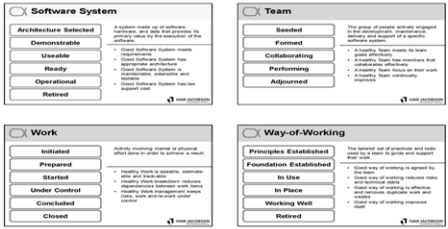
\includegraphics[width=0.5\columnwidth]{img7}\\
Anche il \textit{Work} \textit{le cose da fare} hanno degli stadi ben predefiniti:
\begin{itemize}
	\item \textbf{Initiated:} avere un piano di lavoro;
	\item \textbf{Prepared:} avere un calendario;
	\item \textbf{Started:} partire;
	\item \textbf{Under Control:} sappiamo dove siamo;
	\item \textbf{Concluded:} possiamo dire di aver finito;
	\item \textbf{Close:} risposta degli stakeholders \textit{"va bene"}.
\end{itemize}
Il \textit{Team} deve essere:
\begin{itemize}
	\item \textbf{Seeded:} si comincia a identificare di chi ho bisogno, non come persone ma come competenze. Dobbiamo spersonalizzare, importa il ruolo che ho. Nessuno è un fuoriclasse (perché il fuoriclasse non è disciplinato e sistematico, quindi dannoso), anche se in una buona organizzazione può aiutare (altrimenti fa danno);
	\item \textbf{Formed:} le persone ce le ho e posso lavorare; istituisco dunque tecniche e strumenti per collaborare;
	\item \textbf{Collaborating:} le forme di collaborazione vanno studiate per evitare perdite di tempo;
	\item \textbf{Performed:} una volta acquisite le tecniche siamo efficienti ed efficaci;
	\item \textbf{Adjourned:} "\textit{liberi tutti}", avendo acquisito l'esperienza del lavoro fatto.
\end{itemize}
\end{document}